\subsection{共同目标下的局部最优形状}

令 $r=\log(T/q)$，$w_\kappa=(\rho^\kappa-\E_q\rho^\kappa)/\kappa$，$w_0=C_qr$，于是 $v_\kappa=qw_\kappa$。对固定 Fisher 速度的单位方向 $u_\kappa=v_\kappa/\|v_\kappa\|_F$，reverse KL 的一阶下降量为
\begin{equation}
 -\nabla\KL(q\Vert T)^\top u_\kappa
 =\frac{\E_q[rw_\kappa]}{\sqrt{\E_qw_\kappa^2}}
 \le\sqrt{\Var_qr}.
\end{equation}
这是 Cauchy--Schwarz 不等式，几何形状 $\kappa=0$ 取得等号。对 forward KL，同样有
\begin{equation}
 -\nabla\KL(T\Vert q)^\top u_\kappa
 =\frac{\E_q[\rho w_\kappa]}{\sqrt{\E_qw_\kappa^2}}
 \le\sqrt{\Var_q\rho},
\end{equation}
算术形状 $\kappa=1$ 取得等号。更一般地，$\kappa$ 自己对应的散度具有自己的自然梯度最陡方向。这个局部确定性最优性与平方根形状的最坏矩性质是不同标准，不能由有界方差推出对任何共同评价目标的最优收敛速度。
\subsection{目标自然速度的锐上界与另一个极小极大形状}

对 $0<\kappa<1/2$，令 $X=\rho^\kappa$、$r=1/\kappa>2$，则 $\E_qX^r=1$。写成 $X^2=X^{(r-2)/(r-1)}(X^r)^{1/(r-1)}$，对两因子使用共轭指数 $(r-1)/(r-2)$ 与 $r-1$ 的 Hölder 不等式，得到
\begin{equation}
 \E_qX^2\le(\E_qX)^{(r-2)/(r-1)}
 =(\E_qX)^{(1-2\kappa)/(1-\kappa)}.
\end{equation}
令 $a=\E_qX\in[0,1]$，$\gamma=(1-2\kappa)/(1-\kappa)$。于是 $\Var_qX\le a^\gamma-a^2$。驻点满足 $a^{2-\gamma}=\gamma/2$，代回并记 $b=(1-2\kappa)/[2(1-\kappa)]$，得到锐上界
\begin{equation}
 \boxed{\sup_{q,T}\|v_\kappa\|_F^2
 =C_{\mathrm{vel}}(\kappa)
 =\frac{b^{1-2\kappa}(1-b)}{\kappa^2}}.
\end{equation}
锐性由 $q=(b,1-b)$、$T\to(1,0)$ 达到：$X$ 仅取 $b^{-\kappa}$ 与零，插值不等式和驻点条件同时成立。完整支持分布以极限逼近这个值。$\kappa=1/2$ 的上确界为 4；$\kappa=0$ 或 $\kappa>1/2$ 无有限上界。

在优化 $b$ 后使用包络导数，$d\log C_{\mathrm{vel}}/d\kappa=-2/\kappa-2\log b$。唯一最小点满足
\begin{equation}
 \log\frac{1-2\kappa_\star}{2(1-\kappa_\star)}=-\frac1{\kappa_\star}.
\end{equation}
左侧加 $1/\kappa$ 的导数为 $-1/[(1-2\kappa)(1-\kappa)]-1/\kappa^2<0$，在零点附近趋于正无穷，在 $1/2$ 附近趋于负无穷，故根唯一。根和常数由第一方参考函数 \texttt{minimax\_velocity\_shape}、\texttt{worst\_fisher\_speed\_squared} 计算并验证。

这个最优形状针对 target 的最坏 Fisher 速度上界及小步标量监督方差，与其他拟合散度的误差相关噪声常数最优 $\kappa_{\mathrm{fit}}=1/2$ 是不同标准。更小的最大速度不自动代表更快学习；部分 teacher 方向也可能变慢。平方根的闭式性质和这个极小极大准则都不能替代任务指标。

\begin{figure}[htbp]
 \centering
 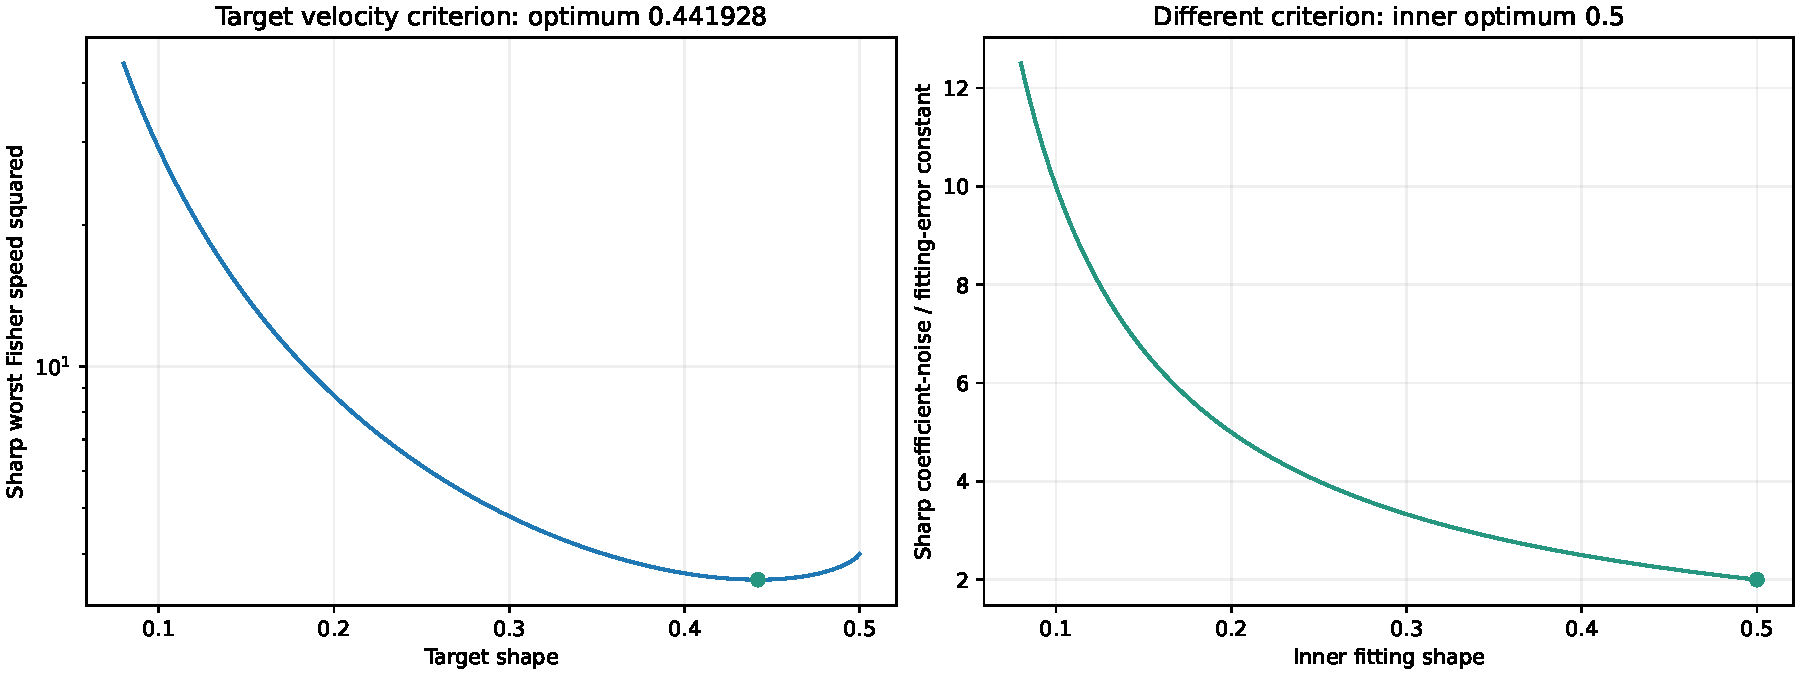
\includegraphics[width=\textwidth]{../../results/power-mean-20261013/two-minimax-criteria.pdf}
 \caption{两个不同的极小极大标准。左图是 target 速度的锐上界，最小点为 $0.441928$；右图是第~\ref{sec:power-projection}~节其他拟合目标的噪声与损失锐相对常数 $1/\kappa_{\mathrm{fit}}$，最小点为 $1/2$。二者都不直接等于最高任务准确率。}
\end{figure}

\subsection{教师误差归一化的锐噪声常数}

\begin{theorem}[平方根形状的相对误差噪声最优性]
\label{thm:power-relative-noise-optimum}
固定 $0<\kappa\le1/2$。令 $\rho=T/q$，小步教师监督为 $A_\kappa^0=(\rho^\kappa-1)/\kappa$，中心为 $K_\kappa^0=[1-\E_q\rho^\kappa]/\kappa$。对至少二元、严格正且 $q\ne T$ 的分布取上确界，有
\begin{align}
 \sup_{q,T}\frac{\Var_qA_\kappa^0}{D_\kappa(T\Vert q)}&=\frac1\kappa,\\
 \sup_{q,T}\frac{\Var_qA_\kappa^0}{K_\kappa^0}&=\frac1{\kappa(1-\kappa)}.
 \label{eq:power-relative-noise-sharp}
\end{align}
在 $\kappa\in[0,1]$ 的幂散度族内，两个准则都由 $\kappa=1/2$ 唯一最小化，锐常数分别为 2 和 4。端点零与 $\kappa>1/2$ 没有有限的统一相对误差常数。
\end{theorem}

\begin{proof}
第~\ref{thm:center-advantage-variance}~定理证明了 $\Var_q(\rho^\kappa)\le[1-a_\kappa]/(1-\kappa)$。除以 $\kappa^2$，再使用 $D_\kappa=[1-a_\kappa]/[\kappa(1-\kappa)]$ 与 $K_\kappa^0=[1-a_\kappa]/\kappa$，得到两个上界。

取 $q=(v,1-v)$、$T=(v^2,1-v^2)$，$v\to0$，则 $\rho=(v,1+v)$。对固定 $0<\kappa\le1/2$，
\begin{equation}
 a_\kappa=v^{1+\kappa}+(1-v)(1+v)^\kappa
 =1-(1-\kappa)v+o(v).
\end{equation}
同理 $a_{2\kappa}=1-(1-2\kappa)v+o(v)$，于是
\begin{equation}
 \Var_qA_\kappa^0=v/\kappa^2+o(v),\quad
 D_\kappa=v/\kappa+o(v),\quad
 K_\kappa^0=(1-\kappa)v/\kappa+o(v).
\end{equation}
相除逼近两个上界，证明锐性。两个常数在 $(0,1/2]$ 上严格递减，最小值均在 $1/2$。

若 $1/2<\kappa<1$，取 $q=(v,1-v)$、$T=(1/2,1/2)$，监督方差按 $v^{1-2\kappa}$ 发散，而 $D_\kappa$ 和 $K_\kappa^0$ 有统一上界。$\kappa=1$ 时方差按 $1/v$ 增长，forward KL 只按 $\log(1/v)$ 增长，且 $K_1^0=0$。$\kappa=0$ 时固定非对称正 $q$，使一个教师概率趋零，方差按平方 log 增长，reverse KL 只按一次 log 增长。故其余形状不存在有限统一常数。
\end{proof}

这个最优性比较的是误差相关噪声常数，并非绝对噪声常数 $C_{\mathrm{vel}}$。所有 $D_\kappa$ 已采用同一局部 Fisher 规范化；其全局值仍随 $\kappa$ 改变。平方根使噪声相对于自身教师误差的最坏放大最小，不意味着每个输入上的方差或任务正确率都最优。
